\documentclass[12pt]{article}
\usepackage[T1]{fontenc}
\usepackage{a4wide}
\usepackage{boxedminipage,color}

\title{Exponential smoothing and change point
  detection}
\author{S�ren H�jsgaard}
\def\eref#1{(\ref{eq:#1})}
\def\DS{S^{[2]}}

\usepackage{Sweave}
\begin{document}
\maketitle
\parindent0pt\parskip5pt

 %s�t dir til "fig" og prefix til "bar" for figurer
\setkeys{Gin}{width=0.9\textwidth} %s�t figurst�rrelse i Sweave
\renewenvironment{Schunk}{\linespread{.85}\scriptsize}{}

%% Efter preamble
\definecolor{myGray}{rgb}{0.95,0.95,0.95}
\makeatletter
\renewenvironment{Schunk}{
  \begin{lrbox}{\@tempboxa}
    \begin{boxedminipage}
      {\columnwidth}\scriptsize}
    {\end{boxedminipage}
  \end{lrbox}%
  \colorbox{myGray}{\usebox{\@tempboxa}}
}
\makeatother

\section{Introduction}
\label{sec:intro}

\begin{Schunk}
\begin{Sinput}
> source('../../EsmoothFUN.R')
\end{Sinput}
\end{Schunk}



The overall goal is to detect indications of mastitis in dairy cows on
the basis of multivariate time series of indicators (the enzyme LDH,
somatic cell counts, electrical conductivity...).  The detection must
be made online meaning only allowed to use past and current data (but
not future data, as would be tempting in connection with various
smoothing methods). When a cow does not have mastitis the indicators
are roughly stationary over time. Mastitis typically implies a jump in
the value of the indicators to a new level, but it is also possible to
see a slower increase. Sometimes the measurements will show an abrupt
change - but only for one or two measurements. This may well be due to
an erroneous recording and hence it is important to be able to
distinguish such (abnormal) short level changes from a real change in
level. 
We want to investigate if exponential smoothing can be used for
distinguishing between 1) normal behaviour, 2) an abrupt change in
level and 3) a slower trend for online data. 


\section{Simple exponential smoothing}
\label{sec:ses}

Given is a time series \{x(t)\} observed at discrete equidistant
times, $t=0,
1,\dots,T$. 
Exponential smoothing or single exponential smoothing (hereafter SES) is a dynamic smoothing of data
which for $0<\alpha<1$ is defined as
\begin{equation}
  \label{eq:es1}
  S(t) 
  = \alpha x(t) + (1-\alpha) S(t-1)
  = S(t-1) + \alpha (x(t)-S(t-1))
\end{equation}

Suppose that the underlying process is ``almost constant'', that is
\begin{displaymath}
  x(t) = a
\end{displaymath}
Then the 
forecast of $x$ at time $t+h$ based on data upto (and
including) time $t$ is
\begin{equation}
  \label{eq:es2}
  \hat x(t+h|t) = S(t)
\end{equation}

For convenience we write $\hat x(t|t)=S(t)$ as $\hat x(t)$ which we
may think of as the current fitted value. 
Notice that
(\ref{eq:es1}) also reads $S(t)=S(t-1) + \alpha e(t)$ where
$e(t)=x(t)-S(t-1)=x(t)-\hat x(t|t-1)$ is the forecast error. 


Rather than the recursive definition of SES in (\ref{eq:es1}) we may
write $S(t)$ as a linear function of data. Letting $\beta=1-\alpha$ we
get
\begin{equation}
  \label{eq:es3}
  S(t) = \alpha \sum_{k=0}^{t-1} \beta^kx(t-k) + \beta^t x(0)
\end{equation}

Two things are clear from (\ref{eq:es3}): First, for large $t$, the influence
of the initial value becomes negligible. Secondly, the sequence of weights
$(\alpha, \alpha\beta, \alpha\beta^2, \dots, \alpha\beta^{t-1})$
decrease exponentially and sum to one. Hence $S(t)$ can be regarded as
a probability weighted average of data (an estimate of the mean $a$)
where recent observations carry the highest weight. 

In practice a value for $\alpha$ must be chosen. A data--driven way is
to choose $\alpha$ so as to minimize sum of squares of 1--step ahead
forecasts, that is: 
\begin{displaymath}
  \sum_{t=2}^T (x(t)-\hat x(t|t-1))^2
\end{displaymath}




\section{Double exponential smoothing}
\label{sec:des}


Double exponential smoothing (hereafter DES) is SES applied to $S(t)$,
that is
\begin{equation}
  \label{eq:des1}
  \DS(t) = \alpha S(t) + (1-\alpha)\DS(t-1)
\end{equation}

Suppose that the true process is ``almost linear'', that is
\begin{displaymath}
  x(t) = a + b t
\end{displaymath}
Then SES will be biased in the
sense that 
\begin{equation}
  \label{eq:des3}
  x(t) - S(t) = b \beta/\alpha \mbox{ for }  t\rightarrow \infty 
\end{equation}
that is $S(t)= a  - b \beta/\alpha + bt =\tilde a + bt$ for large $t$. 
Consequently, if $x(t) = a + b t$ we have by the same argument that $\DS(t) = \tilde
a  - b \beta/\alpha + bt = a  - 2b \beta/\alpha + bt$ for
$t\rightarrow\infty$. Hence $\DS(t)-S(t) \rightarrow b \beta/\alpha$.
From these considerations and \eref{des3} we therefore have 
\begin{eqnarray}
  \label{eq:ses4}
  b &=& (S(t)-\DS(t))\alpha/\beta  \\
  x(t) &=& S(t)- b\beta/\alpha = S(t)+(S(t)-\DS(t))=2S(t)-\DS(t)
\end{eqnarray}

Hence natural estimates of levels and slopes become
\begin{eqnarray}
  \label{eq:des6}
    \hat x(t)  &=& S(t)+(S(t)-\DS(t))=2S(t)-\DS(t)\\
    \hat b(t)    &=& (S(t)-\DS(t))\alpha/\beta
\end{eqnarray}

Similarly, the forecasts become
\begin{equation}
  \label{eq:des7}
  \hat x(t+h|t) = \hat x(t) + \hat b(t) h
\end{equation}


\section{Diagnosis}
\label{sec:diagnosis}

In the following we will denote fitted values from SES by $x_0()$ and
from DES by $x_1()$ (refering to 0'th and 1'st degree polynomials). 

A slow growth can in principle be detected by testing if $b=0$. If we
assume the 


\newpage

\section{Examples}
\label{sec:examples1}

Consider the following scenarios: 1) steady state, 2) abrupt level
change 3) an outlier and 4) a gradual change. Black lines are fitted
values from SES, red lines are from DES. 



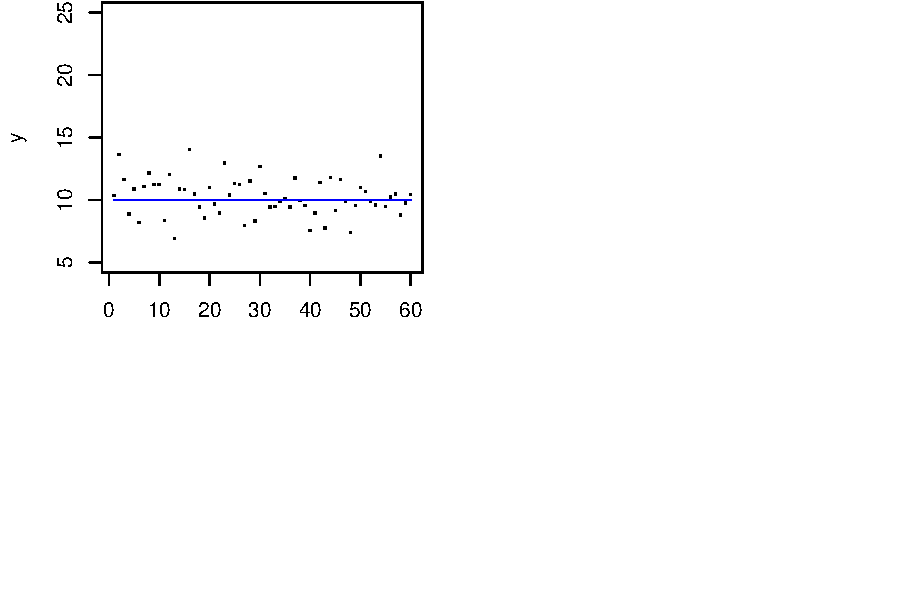
\includegraphics{fig/ES-003}

\newpage


% @ 
% <<forec,eval=F,echo=F>>=
% s0 <- .ses(y,alpha=alpha)
% s1 <- .des(y,alpha=alpha)
% plot(y,pch='.',cex=2);vl()
% lines(s1)
% lines(predict(s1,hh=hh),col=2)
% @ %def 


% @ 
% <<fig=T,height=4,echo=F>>=
% hh    <- 1
% par(mfcol=c(2,2), mar=c(1, 4, 0, 1) + 0.1)
% ###########################################

% y<-y1
% ch<-ch1
% <<forec>>
% y<-y2
% ch<-ch2
% <<forec>>
% y<-y3
% ch<-ch3
% <<forec>>
% y<-y4
% ch<-ch4
% <<forec>>
% @ %def 


\newpage

From $\hat x(t)$ and $\hat x(t,t-h)$ (for $h=1$) we 
can perhaps distinguish between scenario 2) and 3): Look at the differences $\hat x(t)-\hat
x(t,t-h)$ (which is the difference in forecast errors): If that
difference is practically zero at time $t+1$ then the extreme observation at
time $t$ is an ``outlier''



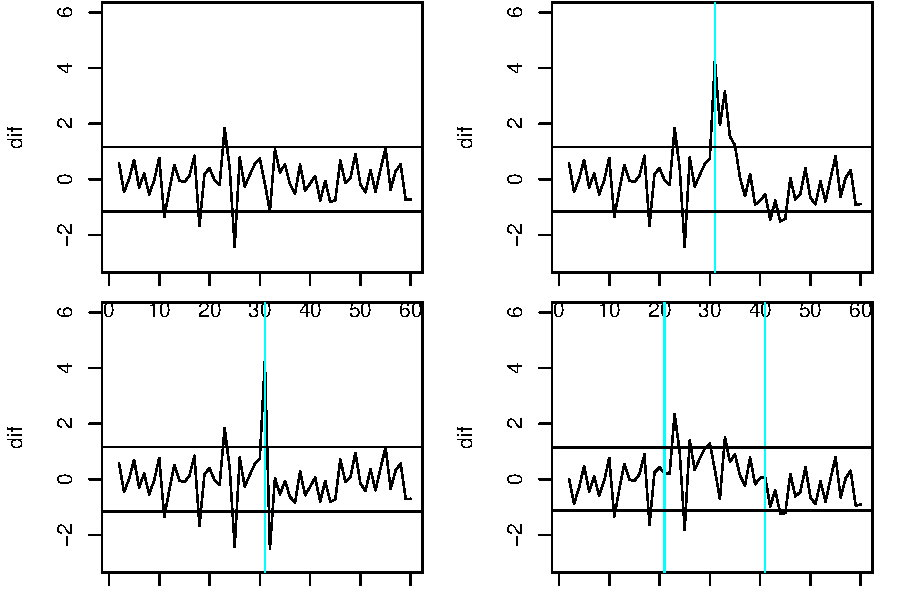
\includegraphics{fig/ES-005}


\newpage 

If we assume data to be stationary at the beginning we can estimate
mean and variance for the level and use this for subsequent tests for
level change. 



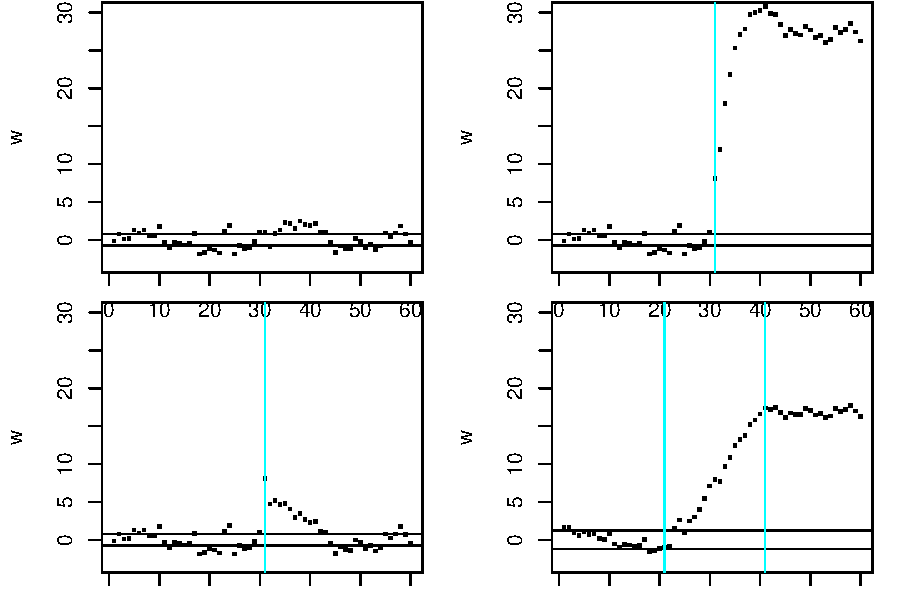
\includegraphics{fig/ES-007}

% w  <- (s1$y-m.y)^2/v.y
% plot(1-pchisq(w,1),pch='.',cex=3)
% abline(h=0.05);vl()











\section{Linear filters and the z--transform}
\label{sec:lfzt}

We can look at \eref{es3} as a linear time invariant filter
\begin{equation}
  \label{eq:es4}
  S(t) = \sum_{j=-\infty}^\infty h(j)x(t-j)
\end{equation}
where $h(j)=\alpha\beta^j$ for $j\ge 0$ and zerp otherwise. Hence  $h(j)$ is
the weight given to $x(t-j)$ in forming $S(t)$ or, equivalently, 
the effect of an observation $x(t)$ at time $t$ will $j$ time steps
later be $x(t)\alpha\beta^j$.

Let $\{h(j)\}$ for $j=-\infty \dots, \infty$
be a collection of weights and define
\begin{equation}
  \label{eq:lf1}
  y(t) = \sum_{j=-\infty}^\infty h(j)x(t-j)
\end{equation}

Then (\ref{eq:lf1}) is a linear time invariant filter. As an example,
suppose that $h(0)$, $h(1)$ and $h(2)$ are non--zero and all other
weights are zero. Then we get
\begin{equation}
  \label{eq:lf2}
  y(t) = h(0) x(t) + h(1)x(t-1) + h(2)x(t-2)
\end{equation}

Equation (\ref{eq:lf1}) is called a convolution of $x()$ and $h()$
and we write this briefly as 
\begin{equation}
  \label{eq:lf3}
  y(t) = x(t)*h(t)
\end{equation}

We want to study what $y(t)$ looks like for different choices of
$x(t)$ and $h(t)$. In doing so we use the z--transform: Let $f(n)$ be
a function defined for integer values of $n$. The z--transform is 
\begin{equation}
  \label{eq:lf4}
  F(z) = \sum_{n=-\infty}^\infty f(n)z^n
\end{equation}
for complex values $z$. Notice that we write the function in lower
case and the  z--transform of the function in upper case. Tables exist
for pairs of functions and their z--transform. 


We apply the z--transform to \eref{lf2}. Change variables from as
$m=t-j$ so that $j=t-m$ so that 
\begin{equation}
  \label{eq:lf5}
  y(n) = \sum_{m=-\infty}^\infty x(m) h(n-m)  
\end{equation}

Now apply the z--transform to $y(n)$ and we get (where all summations
are from $-\infty$ to $\infty$):
\begin{eqnarray}
  Y(z) 
  &=& \sum_n z^n \sum_m x(m) h(n-m) \nonumber \\
  &=& \sum_m \{z^m x(m) \sum_n z^{n-m}  h(n-m)\} \nonumber  \\
  &=& \sum_m \{z^m x(m) \sum_p z^{p}  h(p)\} \nonumber \\
  &=& H(z) X(z)
  \label{eq:lf6}  
\end{eqnarray}

Hence, all we need to do is to find $H()$ and $X()$ (typically by
looking into a table), carry out the
multiplication in \eref{lf6} to find $Y(z)$ and then find $y(t)$ by
looking into the table again.  

There are linearities to be exploited in this connection: If
$f(n)=\sum_u \alpha_u f_u(n)$ then $F(z) =\sum_u \alpha_uF_u(z)$. Thus
if $x(t)= \sum_u \alpha_u(t)$ and $h(j)=\sum_v \beta_v h_v(j)$ then
\begin{equation}
  \label{eq:lf7}
  Y(z) = \sum_{u,v} \alpha_u\beta_v X_u(z)H_v(z) = \sum_s \gamma_s
  Y_s(z),
\end{equation}
say. Exploiting the linearity again then gives
\begin{equation}
  \label{eq:lf8}
  y(t) = \sum_s \gamma_s y_s(t)
\end{equation}

\end{document}

% \subsection{Steady--state}
% \label{sec:xxx}

% @ 
% <<fig=T,height=5,echo=F>>=
% source("EsmoothFUN.q")
% mu <- rep(10,60)
% y  <- mu + eps
% ch <- NA
% <<chunk1>>
% @ %def 

% \subsection{Outlier}
% \label{sec:xxx}

% @ 
% <<fig=T,height=5,echo=F>>=
% mu <- rep(10,60)
% mu[31] <- 20
% y  <- mu + eps
% ch <- 31
% <<chunk1>>
% @ %def 


% \subsection{Abrupt change}
% \label{sec:xxx}

% Now see what happens if the level suddenly changes. 

% @ 
% <<fig=T,height=5,echo=F>>=
% mu <- c(rep(10,30), rep(20,30))
% ch <- 31
% y  <- mu + eps
% <<chunk1>>
% @ %def 


% \subsection{Gradual change}
% \label{sec:xxx}

% Now study what happens when there is a gradual change:

% @ 
% <<fig=T,height=5,echo=F>>=
% mu <- c(rep(10,20), 10+(1:20)/2, rep(20,20))
% ch <- c(21,41)
% y  <- mu + eps
% <<chunk1>>
% @ %def 







% @ 
% <<chunk1,eval=F,keep.source=T,echo=F>>=
% par(mfcol=c(5,2), mar=c(1, 4, 0, 1) + 0.1)

% alpha <- .2
% hh    <- 5
% s0 <- .ses(y,alpha=alpha)
% s1 <- .des(y,alpha=alpha)

% www <- 1:20
% www <- c(1,4,7,11,15,18)
% m.y <- mean(s1$y[www])
% v.y <- var (s1$y[www])
% m.b <- mean(s1$b[www])
% v.b <- var (s1$b[www])

% plot(y, ylim=range(y,s0$y,s1$y));vl()
% lines(s0,col=1)
% lines(s1,col=2)

% rmat <- cbind(resid(s0), resid(s1))
% matplot(rmat, type='l'); vl(); hl()

% ferr<-as.data.frame(cbind(predict(s0,hh=hh)$ferr, predict(s1,hh=hh)$ferr))
% ferr$dif.ferr <- ferr[,2]-ferr[,1]
% matplot(ferr, type='l',lty=1); vl();hl()

% parmest <- do.call(cbind,s1)[,2:3]
% matplot(parmest,type='l',lty=1); vl()
% matplot(scale(parmest),type='l',lty=1); vl()

% parmest2 <- parmest
% parmest2[,1] <- parmest2[,1]/sqrt(v.y)
% parmest2[,2] <- parmest2[,2]/sqrt(v.b)
% matplot(parmest2,type='l',lty=1); vl()

% w.y <- (s1$y-m.y)^2/v.y
% w.b <- (s1$b-m.b)^2/v.b

% p.y <- pchisq(w.y,1)
% p.b <- pchisq(w.b,1)
% ps.y <- pchisq(.ses(w.y)$y,1)
% ps.b <- pchisq(.ses(w.b)$y,1)
% plot(p.y); vl()
% lines(ps.y)
% plot(p.b);vl()
% lines(ps.b)

% db <- c(NA, diff(s1$b))
% m.db <- mean(db[www],na.rm=T)
% v.db <- var(db[www],na.rm=T)
% plot(db,type='l'); vl();hl()
% abline(h=c(m.db, m.db-1*sqrt(v.db), m.db+1*sqrt(v.db)),col=c(4,3,3))
% @ %def 



